\documentclass[10 pt,usenames,dvipsnames, oneside]{article}
\usepackage{../../../modelo-ensino-medio}



\begin{document}

\begin{center}
  \begin{minipage}[l]{3cm}

\includegraphics[width=2cm]{logo}    
\end{minipage}\hfill
\begin{minipage}[r]{.8\textwidth}
 {\Large \scshape Atividade: Frio nas alturas}  
\end{minipage}
\end{center}
\vspace{.2cm}

\ifdefined\prof
\begin{objetivos}
\item \textbf{EM13MAT302} Construir modelos empregando as funções polinomiais de 1º ou 2º graus, para resolver problemas em contextos diversos, com ou sem apoio de tecnologias digitais.
\end{objetivos}

\begin{goals}
\begin{enumerate}
\item Explorar o zero da função afim.
\item Compreender em um contexto específico a importância da determinação do zero da função.
\item Perceber que a altitude de acionamento do sistema anti-gelo (o zero da função) se obtém dividindo o valor da temperatura pelo valor absoluto da taxa de variação.
\end{enumerate}

\tcblower

\begin{itemize}
\item É possível responder à pergunta e) pensando como um problema de progressão aritmética: Se a temperatura local é $30$ $^{\circ}$C e ela diminui $2$ $^{\circ}$C a cada $1.000$ pés, para chegar a zero devemos subtrair $2$ de $30$, um total de $15$ vezes, logo, a altitude é $15.000$ pés.
\item Os itens f) e g) pretendem dar uma ideia de como se obtem a expressão geral do zero da função afim. Caso julgue pertinente, estimule-os a pensar em situações hipotéticas em que as taxas de variação da temperatura em função da altitude sejam diferentem.
\end{itemize}

\end{goals}

\bigskip
\begin{center}
{\large \scshape Atividade}
\end{center}
\fi

Mesmo em pleno verão um avião, precisa lidar com temperaturas muito baixas. Quando uma aeronave opera em baixas temperaturas, com umidade presente, há a possibilidade de formação de gelo que virá a se acumular na sua estrutura ou em seu grupo moto-propulsor. O gelo se forma quando um avião voa através de uma nuvem ou de um ambiente contendo gotículas de água super-resfriadas. O principal problema causado pela formação de gelo é a modificação do fluxo de ar sobre as superfícies das asas, prejudicando assim o desempenho da nave e acarretando, eventualmente, em mais gastos de combustível. Para evitar problemas como esses as aeronaves contam com um sistema anti-gelo que diminui a formação de camadas de gelo em sua fuselagem, produzindo os chamados “rastros de condensação” como na imagem.

\begin{figure}[H]
\centering

\noindent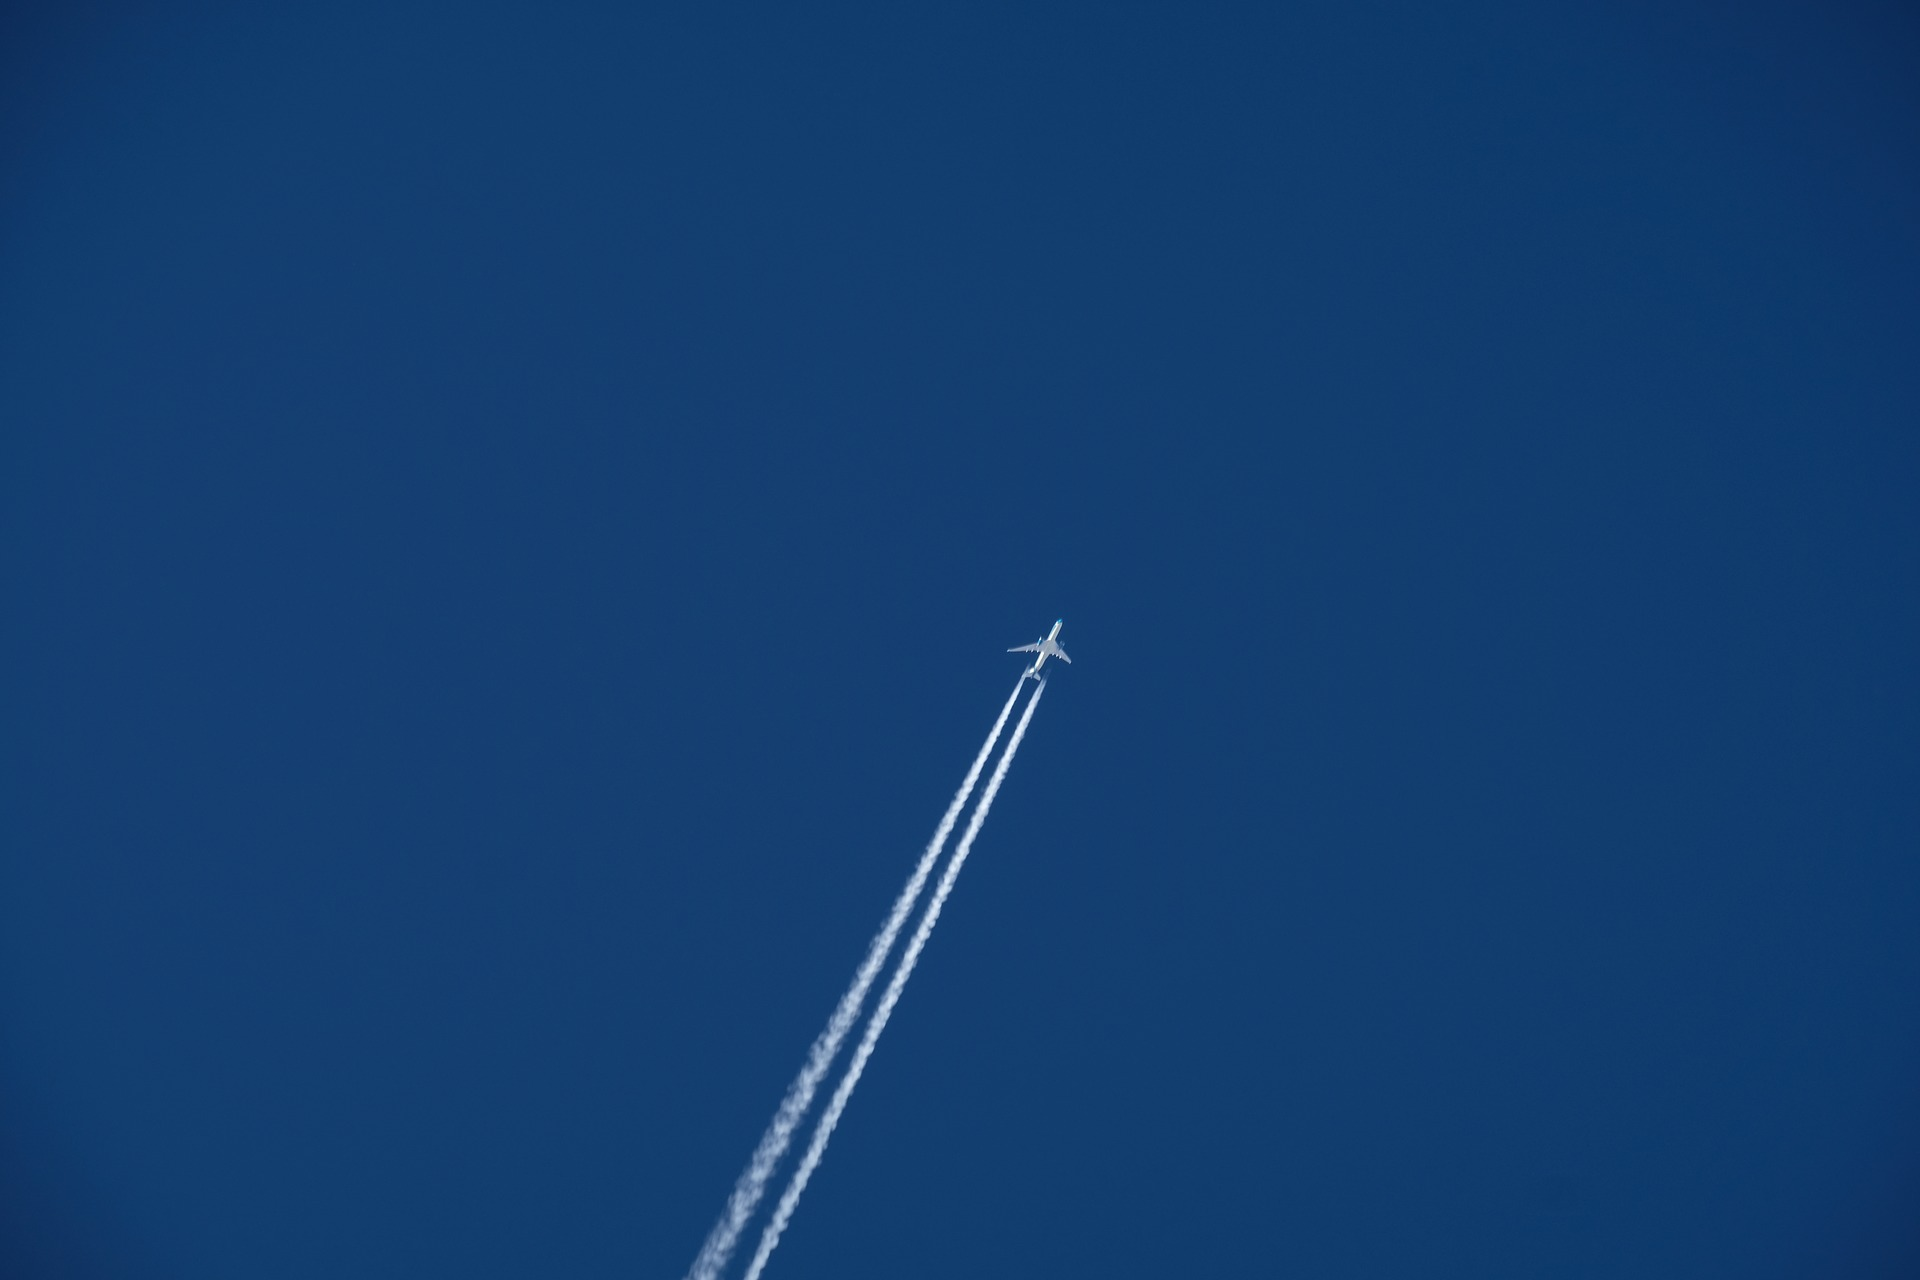
\includegraphics[width=250bp]{frio-aviao.jpg}
\end{figure}

A temperatura na troposfera (primeira camada da atmosfera que tem aproximadamente \(40.000\) pés de altitude) diminui \(2^\circ C\) a cada aumento de \(1.000\) pés na altitude. Suponha que, em um determinado dia, a temperatura em um aeroporto seja de \(30^\circ C\), e que a água congela a \(0^\circ C\).
\begin{enumerate}
\item {} 
Qual a taxa de variação, em \(^\circ C/\text{pé}\), da temperatura da atmosfera, \(T\), em função da altitude, \(h\).

\item {} 
A função \(T(h)\) é crescente ou decrescente? Como isso se reflete na taxa de variação?

\item {} 
Determine uma expressão para \(T(h)\) e represente seu gráfico.

\item {} 
Qual a temperatura a \(37.200\) pés de altitude?

\item {} 
A partir de que altitude o piloto deverá acionar o sistema anti-gelo da aeronave?

\item {} 
Em outro dia, a temperatura no mesmo aeroporto era de \(25^\circ C\). Qual a altitude de acionamento do sistema anti-gelo, nesse caso?

\item {} 
Estabeleça uma maneira de calcular a altitude de acionamento do sistema anti-gelo quando a temperatura do aeroporto é igual a \(T_0\).

\end{enumerate}

\ifdefined\prof
\begin{solucao}
\begin{enumerate}

\item $−0{,}002$ $^{\circ}$C/pé
\item $T$ é decrescente, portanto a taxa de variação é negativa.
\item $T(h)=30−0{,}002h$
\item $T(37.200)=−44{,}4$ $^{\circ}$C
\item $15.000$ pés
\item $12.500$ pés
\item Nesse caso, $T(h)=T0−0,{,}02h$. Para determinar a altitude, basta calcular $h$ para o qual se tem $T(h)=0$, isto é, $h=\displaystyle\frac{T_0}{0{,}002}=500T_0$
\end{enumerate}
\end{solucao}
\fi

\end{document}